\begin{frame}{Greedy}
    \begin{center}
        \begin{lemma}
            $$f(G) \geq (1 - e^{-\frac{|G|}{|O|}})f(O)$$
        \end{lemma}
        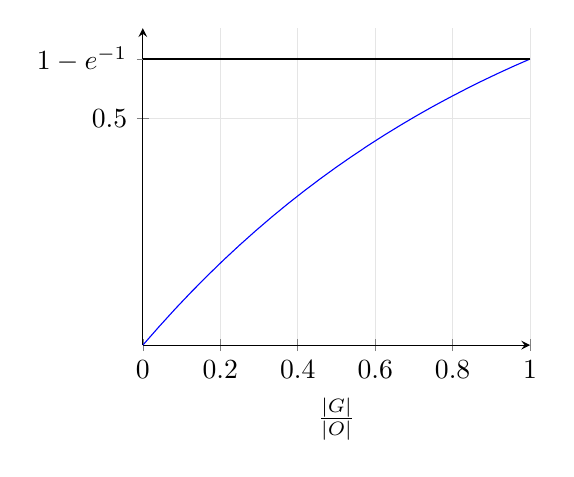
\begin{tikzpicture}[every node/.style={}]
            \begin{axis}[
                domain=0:1
                ,width=6.5cm
                ,ymax=.7
                ,xlabel=$\frac{|G|}{|O|}$
                ,axis lines=left
                ,grid=both
                ,grid style={
                        draw=gray!20
                }
                ,ytick={0.5}
                ,extra y ticks={
                    0.632120558829
                }
                ,extra y tick labels={$1 - e^{-1}$}
            ]
                \addplot[blue]{1-exp(-(x))};
                \addplot[thin]{1-exp(-1)};
            \end{axis}
        \end{tikzpicture}
    \end{center}
\end{frame}